\begin{figure*}
    \centering
    \begin{subfigure}[h]{0.45\textwidth}
        
        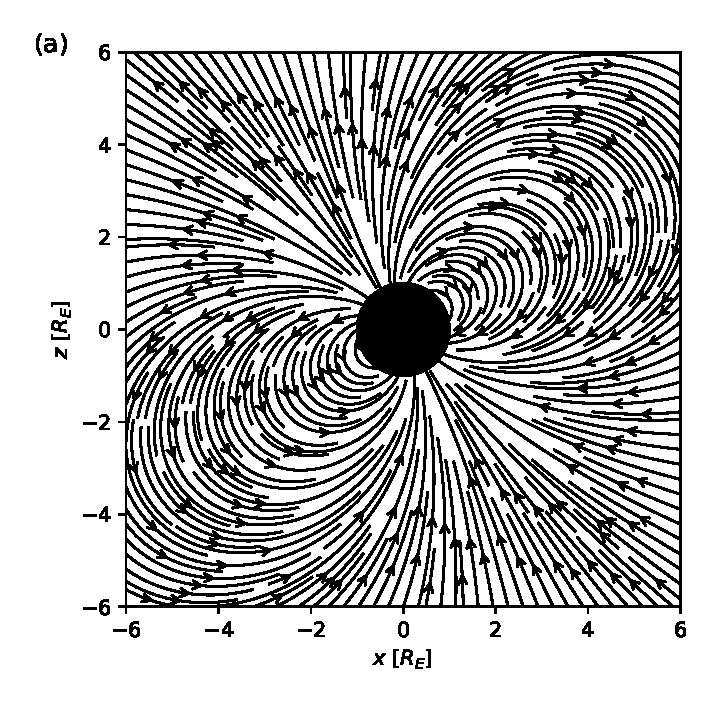
\includegraphics[width=\textwidth]{Figures/BField/magnetic-field-lines-x0z.eps}
        \label{fig:xz}
    \end{subfigure}
    \hfill
    \begin{subfigure}[h]{0.45\textwidth}
        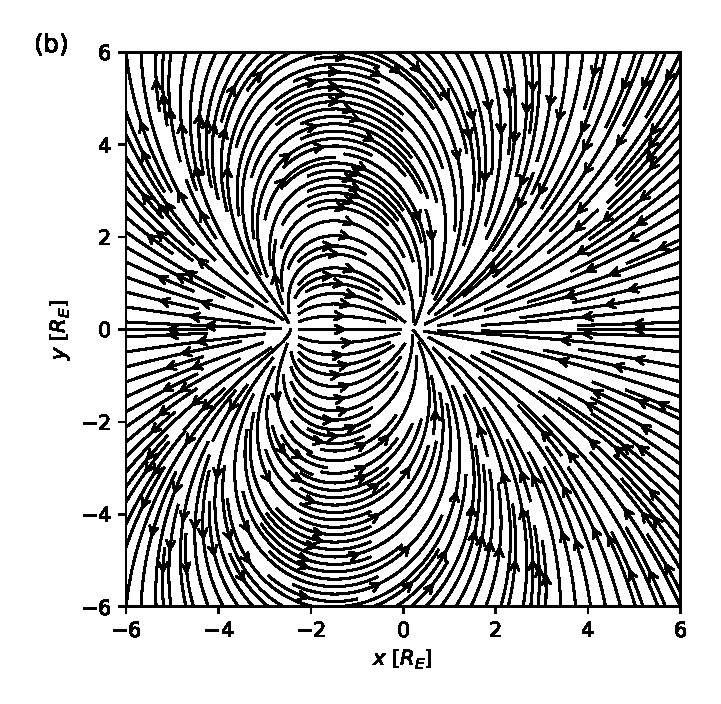
\includegraphics[width=\textwidth]{Figures/BField/magnetic-field-lines-xy-1.eps}
        \label{fig:xy}
    \end{subfigure}
    \caption{Streamline plots of the magnetic field lines computed via equation (\ref{eq:B-field-cart}). (a): The magnetic field lines in the $xz$-plane at $y=0$. The black circle indicates the Earths. (b): The magnetic field lines in the $xy$-plane at $z=-1R_E$. The magnetic equator is tilted around the $y$-axis towards the sun, i.e in the negative $x$-direction}
    \label{fig:B-field}
\end{figure*}